\begin{frame}{Bewusstsein als Aggregatzustand}
	\begin{columns}
		\begin{column}{0.55\textwidth}
			\begin{itemize}
				\item{Aggregatzustände durch Eigenschaften unterscheidbar}
				\item{Ähnliche Konzepte bereits erdacht}
				\begin{itemize}
					\item{\emph{Computronium}}
				\end{itemize}
				\item{Welche Eigenschaften muss \emph{Perceptronium} besitzen?}
			\end{itemize}
		\end{column}
		\begin{column}{0.45\textwidth}
			\centering
			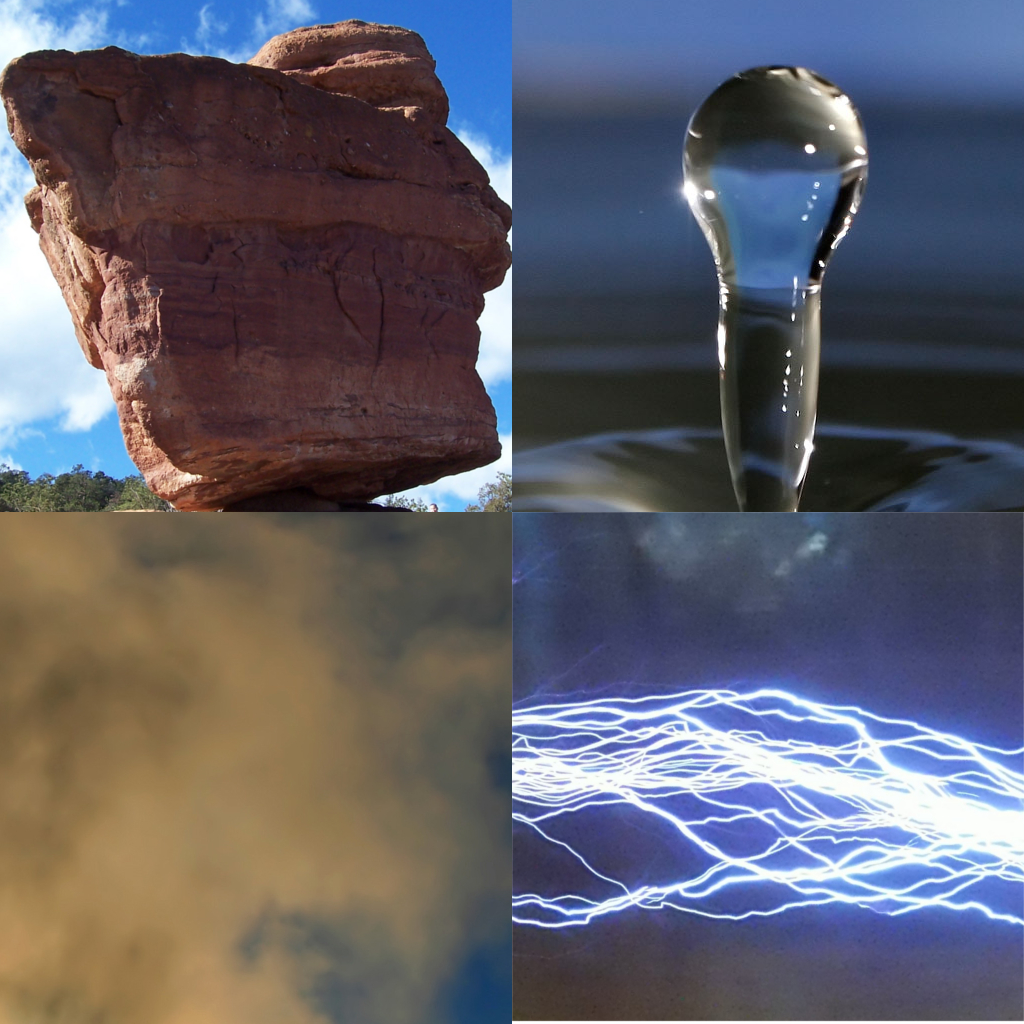
\includegraphics[scale=0.15]{graphics/states_of_matter.jpg}\\\hfill\cite{pic_stone,pic_water_droplet,steam_eruption,lightning_teslacoil}
		\end{column}
	\end{columns}
\end{frame}